\section{Eksperimenti 2. faze}
Z laboratorijskimi eksperimenti v 1. fazi smo dobili zadovoljive rezultate, težave pa so nastale pri uporabi postopka na terenu. Zato smo v 2. fazi optimizirali posamezne segmente elementarnega postopka estimacije fizioloških parametrov. Te smo tudi uporabili v končni preiskavi. V preliminarnih testih so opisani tudi drugi postopki, ki smo jih potrebovali zaradi uporabe Kinect kamer.

Za statistično bolj oprijemljive rezultate smo v laboratorijskih in terenskih eksperimentih 2. faze uporabili 7 različnih merjencev z oznakami: SUBJ1, SUBJ2, SUBJ4, SUBJ7, SUBJ8, SUBJ9, SUBJ10. 

Merjenca SUBJ4 smo uporabili samo v laboratorijskih eksperimentih, ker pri terenskih eksperimentih ni bil prisoten. Namesto njega smo v terenskih eksperimentih uporabili merjenca SUBJ10. V laboratorijskih eksperimentih merjenca SUBJ10 nismo upoštevali zaradi napak pri zajemu meritev.

Med laboratorijskimi in terenskimi eksperimenti je za merjenca SUBJ1 in SUBJ2 preteklo 43 dni, za merjenca SUBJ4 42 dni in za ostale 1 dan.  

\subsection{Preliminarni testi}
\subsubsection{Združevanje slik iz dveh Kinect kamer}\label{sec:zdruzevanje}

\paragraph{Združevanje z značilkami}
Časovno sinhornizirana zaporedja slik smo poskušali združiti z metodo panoramskega šivanja slik z uporabo značilk, kot je opisano v delu \cite{brown2007automatic}. Tu smo namesto SIFT značilk uporabili SURF značilke.


\paragraph{Združevanje s kontrolnimi točkami}
Zaporedja slik smo poskušali združiti z ročnim določevanjem kontrolnih točk.


\paragraph{Prilagojeno združevanje}
Zaradi nezadovoljivih rezultatov klasičnih metod združevanja stereo slik, smo razvili metodo, ki je prilagojena za Kinect kamere. Iz kamer smo pridobili intrinzične parametre infra-redečega (IR) senzora, in sicer: slikovni koordinati goriščne razdalje $f_u$ in $f_v$ ter slikovni koordinati optičnega središča slike (ang. principal point) $c_u$ in $c_v$. Intrinsične parametre smo uporabili za določitev intrizične matrike $\vec{M}_{int}$ po enačbi \eqref{eq:intrinsic}.


Ker pravih ekstrinsičnih parametrov kamer nismo poznali, smo jih le ocenili z metodo določevanja sečišča vidnih polj obeh kamer. Sečišče je prikazano kot rdeča linija na sliki \ref{fig:zdruzevanje}. S to metodo smo določili translacijski vektor $\vec{t} = \left [ t_x~ t_y~ t_z \right]^\top$ in rotacijsko matriko $\vec{R}$ iz Eulerjevih kotov.

S sledenjem igralca z DS-KCF algoritmom, smo s pomočjo projekcijske matrike \eqref{eq:projection-matrix} določili center tarče v metričnih enotah za vsako sliko zaporedja leve in desne kamere. Kadar slikovni element ni vseboval podatkov globine, smo za center tarče izbrali najbližji slikovni element z veljavno globino.

Prva slika združenega zaporedja je bila slika kamere, kjer se igralec prvič pojavi. Nadaljne slike smo izbirali med zaporedjema kamer glede na pozicijo centra tarče. Ko je šel center tarče skozi upragovljeno mejo, ki je na sliki \ref{fig:zdruzevanje} prikazana z modro linijo smo preklopili na drugo kamero. Razdalja med pragom in sečiščem je znašala \SI{200}{mm}.


\begin{figure}[htb]
	\centering
	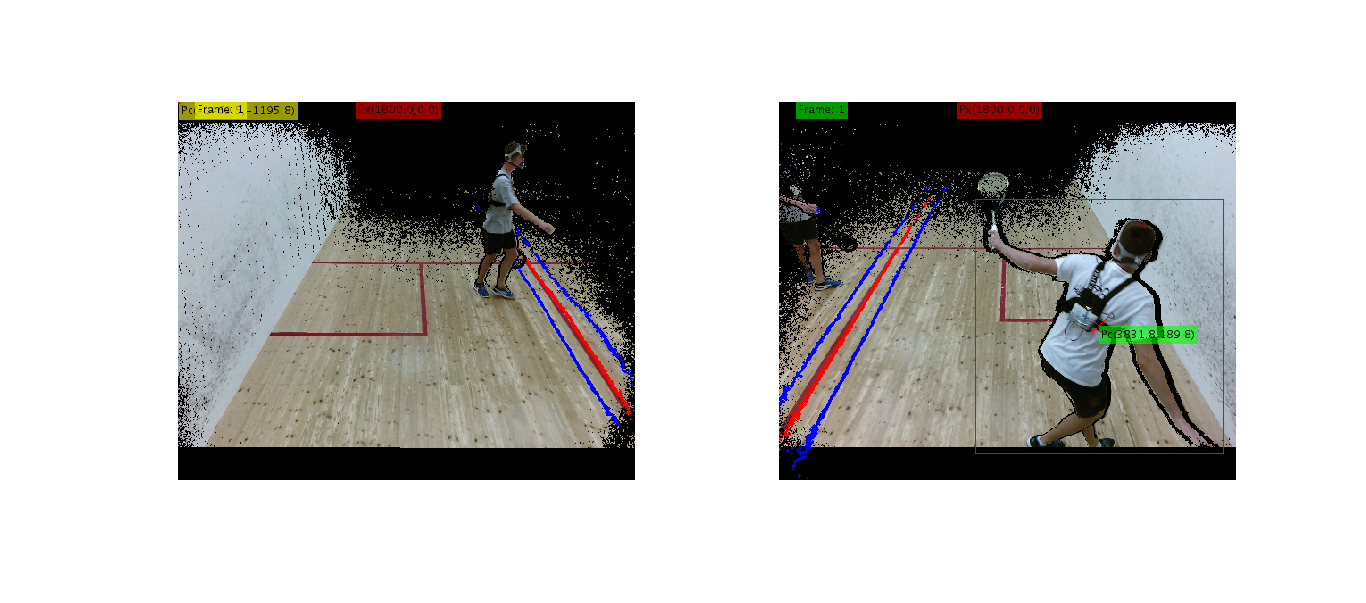
\includegraphics[width=\columnwidth]{./Slike/zdruzevanje-example.png}
	\caption[Določevanje sečišča vidnih polj leve in desne Kinect kamere]{Določevanje sečišča vidnih polj leve in desne Kinect kamere. Na sliki sta prikazani prvi sliki zaporedja leve in desne Kinect kamere 1. seta 2. igre terenskega eksperimenta iz 2. faze. Označen je 4. igralec. Zelena barva koordiat središča tarče predstavlja izbrano kamero. Kamera z rumeno barvo ni izbrana. Sečišče je rdeča linija. Modri liniji sta pragova za preklop med kamerama. Ležita \SI{200}{mm} levo in desno od sečišča.}
	\label{fig:zdruzevanje}
\end{figure}



\subsubsection{Mrežno iskanje \texorpdfstring{$\nu$}{nu}-RBF}
Med evaluacijo eksperimentov 1. faze smo ugotovili, da z regresijo \esvr pogosto dobimo preobremenjene (ang. Overfitted) modele. Pri takih modeli je število podpornih vektorjev zelo visoko. Lahko se zgodi, da postanejo vsi vektorji značilk podporni vektorji. Preobremenjeni modeli lahko dajejo solidne rezultate, vendar pa so ti nerealistični. Takoj, ko bi v tak model vnesli rahlo spremenjene podatke, ne bi več delovali.

Zaradi tovrstnih problemov smo v našem postopku regresijo \esvr zamenjali z \nusvr. Izkazalo se je, da tudi ta ne deluje, čeprav pri njej uporabljamo dodatni parameter $\nu$, s katerim v teoriji kontroliramo razmerje števila podpornih vektorjev, kot je opisano v poglavju \ref{sec:regresija-nusvr}. Chang et. al nam v delu \cite{chang2002training} parameter $\nu$ bolj natačno opiše kot spodnjo mejo razmerja števila podpornih vektorjev. Parameter $\nu$ tako v resnici ne predstavlja omejitve, s katero bi kaznovali prekomerno učneje modela. V ta namen smo razvili mrežno iskanje \nurbf, ki je predstavljeno v poglavju \ref{sec:nurbf}. 

Razvito mrežno iskanje \nurbf uporablja regresijo \nusvr in jedro RBF, zato smo ju uporabljali tudi za učenje modelov. Celoten postopek krajše imenujemo kar \nurbf.

\paragraph{Optimizacija parametrov}
Najprej smo optimizirali parameter $\numax$ oziroma $\numax'$. Slednji predstavlja različico parametra $\numax$, s katerim določimo dejansko število podpornih vektorjev. Za tovrstno optimizacijo smo ponovno naučili \textit{mixed} modele iz 1. faze, pri čemer smo za mrežno iskanje uporabili nov postopek. Modele smo nato uporabili za testiranje na učnih podatkih terenskih eksperimentov 1. faze. S takim postopkom smo izluščili slabe \textit{squash} modele, ki bi oteževali pravilno evaluacijo rezultatov pri optimizaciji.

Za optimizacijo smo uporabili HOOF-HAFA deskriptor in naslednje vrednosti parametrov: začetna vrednost $\nu$ $0.1$ in standardni odklon za Gaussov filter $\sigma=5$. Za $\numax'$ smo uporabili 400, 800 in 1200 podpornih vektorjev. 

Z optimiziranim parametrom $\numax'=400$ smo \nurbf preizkusili še na elementarnih modelih. Tu smo za razliko od eksperimentov iz 1. faze poleg \nurbf uporabili razširjeni HOOF-HAFA deskriptor.







\subsubsection{Jedro GHI}
V poglavju \ref{sec:ghi} smo opisali, da je jedro GHI primerno za histogramske deskriptorje, zato smo ga tudi preizkusili na elementarnih modelih. Tu smo namesto prvotnega HOOF deskriptorja uporabili HOOF-HAFA deskriptor, ki daje boljše rezultate. Pri uporabi GHI jedra smo značilke skalirali na intervalu $[-1,~1]$ zaradi hitrejšega učenja. Učili smo z \esvr metodo. Rezultate smo filtrirali s prvotnim Kalmanovim filtrom.

Zaradi že prej omenjenih težav s prevelikim številom podpornih vektorjev v modelih, smo pri klasičnem mrežnem iskanju sprva uporabili enostavno mero: faktor števila podpornih vektorjev $f_{nSV}$, ki je opisan z enačbo \eqref{eq:fnsv}. $n_v$ je število vzorcev in $n_{SV}$ je število podpornih vektorjev. S to mero določimo procentualno vrednost vektorjev, ki lahko postanejo podporni. Zaradi tega faktorja optimizacija parametra regresije ni bila potrebna. Pri testiranju smo uporabili vrednost $f_{nSV} = 0.01$.


\begin{equation}
f_{nSV} = \frac{n_v - n_{SV}}{n_v}
\label{eq:fnsv}
\end{equation} 

Zgoraj opisana metoda ni delovala zato smo namesto faktorja $f_{nSV}$ uporabili postopek \nughi. Gre za prilagojeno različico postopka \nurbf, kjer smo uporabili GHI jedro. Dodatna razlika je še v tem, da predikcij pri križni validaciji nismo filtrirali, ker smo pri rezultatih uporabili Kalmanov filter. Prav tako smo s tem zagotovili zadovoljiv čas reševanja problema.






\subsubsection{Optimizacija Gaussovega filtra}
Pri optimizaciji Gaussovega filtra smo določili optimalni standardni odklon $\sigma$ z uporabo dveh metrik, in sicer: koren srednje kvadratične napake (RMSE) in razmerje med signalom in šumom (SNR). Pri RMSE metriki smo določili napako med učnimi vzorci in njihovo predikcijo. Pri SNR metriki smo za signal uporabili referenčne učne vzorce. Za šum smo uporabili rezidualni ali preostali šum. Tega smo dobili z odštevanjem filtriranih vzorcev od referenčnih. SNR metrika tako določa uspešnost izločevanja šuma, RMSE metrika pa pravilnost določevanja kateri podatki spadajo v signal in kateri v šum.


Teste smo izvajali na vseh eksperimentih 1. sklopa, pri čemer smo uporabili \nurbf mrežno iskanje s \SI{50}{\%} podpornih vektorjev. Za filtriranje pri mrežnem iskanju smo izbrali najmanjši filter s $\sigma = 1$. Testirali smo naslednje standardne odklone Gaussovega filtra: $1, 3, 5, 11, 21, 31$ in $51$. 




\subsubsection{Normalizacija HAFA deskriptorjev}
V praksi se pokaže, da prvotni HAFA histogram ne deluje zadovoljivo, saj se histogram lahko močno spreminja pri uporabi sledilnika. Zaradi neidelanega delovanja sledilnika področje tarče skozi čas spreminja svojo velikost, to pa vpliva na vrednosti stolpcev HAFA histograma. Ker te dobimo s preštevanjem slikovnih elementov z enako amplitudo hitrosti bo manjše področje posledično zmanjšalo celoten histogram. Pri HOOF histogramih tega problema praktično nimamo, saj ima majhen vpliv. Razlog tiči v računanju vrednosti stolpcev HOOF histograma. Njihove vrednosti dobimo s seštevanjem amplitud in ne njihovim preštevanjem. Te so zato pred normiranjem praviloma večje.

Probleme sledilnika smo poskušali kompenzirati z uvedbo amplitudnega faktorja $f_A$. Amplitudni faktor je pravzaprav razmerje med velikostjo področja igralca na terenskih testih in velikostjo merjenca na tekalni stezi. Razmerje lahko preprosto dobimo z razmerjem diagonal področij po enačbi \eqref{eq:diag}, kjer so $w_l$ in $h_l$ širina in dolžina področja na tekalni stezi ter $w_s$ in $h_s$ širina in dolžina področja na terenskih testih.

\begin{equation}
f_A = \frac{\sqrt{w_l^2 + h_l^2}}{\sqrt{w_s^2 + h_s^2}}
\label{eq:diag}
\end{equation}

Velikost diagonale na laboratorijskih testih uporabljamo kot referenco. To pa zato, ker je na teh posnetkih stabilna, saj se le malo spreminja. Koncept amplitudnega faktorja smo preizkusili na enakem postopku, kot pri optimizaciji parametra mrežnega iskanja \nurbf. S takim postopkom smo izluščili slabe \textit{squash} modele, ki bi oteževali pravilno evaluacijo rezultatov pri optimizaciji. Naučili smo modele \textit{diag}, kjer smo uporabili amplitudni faktor in referenčne modele \textit{normal} brez uporabe faktorja za primerjavo. Diagonalo na tekalni stezi smo določili po sliki \ref{fig:diag-bbox}, kjer smo za zgornji levi kot $P_0$ in spodnji desni kot $P_1$ izbrali vrednosti v tabeli \ref{tab:diag}. 


\begin{figure}[htb]
	\centering
	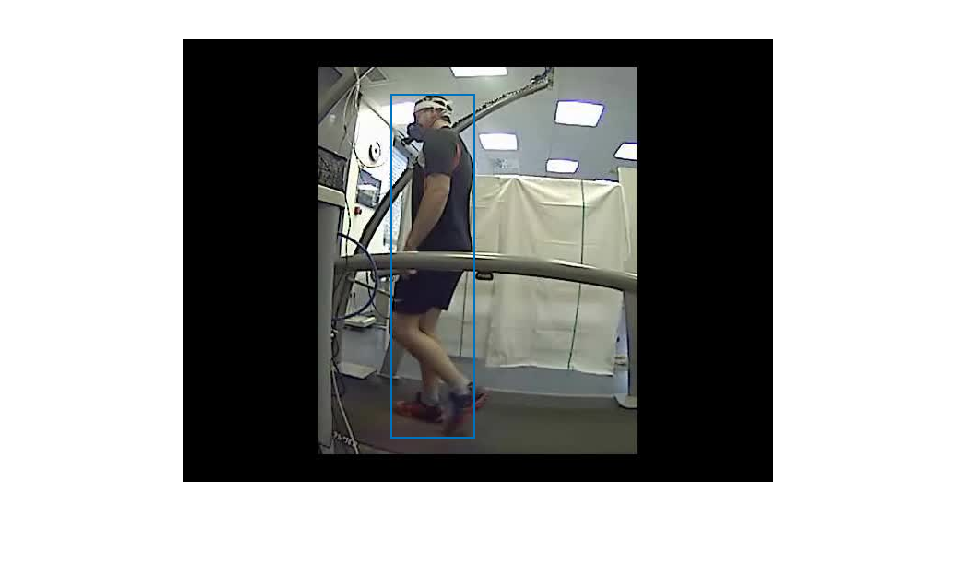
\includegraphics[width=0.75\columnwidth]{./Slike/diag-bbox.png}
	\caption{}
	\label{fig:diag-bbox}
\end{figure}

\begin{table}[htb]
	\centering
	\begin{tabular}{l S[table-format=3] S[table-format=3]}
		\toprule
		\textbf{Točka} & \thead{$\mathbf{x}$} & \thead{$\mathbf{y}$} \\ 
		\midrule
		$P_0$ & 297 & 82 \\
		$P_1$ & 389 & 452 \\
		\bottomrule
	\end{tabular}
	\caption[Optimalni parameteri RBF jedra modelov za izbiro deskriptorjev]{Optimalni parametri RBF jedra za modele z različnim deskriptorjem.}
	\label{tab:diag}
\end{table}

Pri testiranju smo uporabili parameter $\numax$ \SI{50}{\%} podpornih vektorjev. Za Gaussov filter smo uporabili $\sigma=5$. Značilke smo skalirani na intervalu $[0,~1]$. Za modele z diagonalo smo uporabili parameter $f_{A}=381.266$. Pri učenju smo uporabili optimalne vrednosti parametrov, ki so prikazane v tabeli \ref{tab:diag}. Za evaluacijo rezultatov smo uporabili predikcije testnih vzorcev z modeli s zakasnitvijo.



\begin{table}[htb]
	\centering
	\begin{tabular}{l S[table-format=3] S[table-format=1.3] S[table-format=1.1] S[table-format=1.3]}
		\toprule
		\textbf{Model} & \thead{$\mathbf{C}$} & \thead{$\mathbf{\gamma}$} & \thead{$\mathbf{\nu}$} & \thead{MSE} \\ 
		\midrule
		NORMAL & 256 & 0.354 & 0.1 & 5.297 \\
		DIAG & 256 & 0.354 & 0.1 & 5.297 \\
		\bottomrule
	\end{tabular}
	\caption[Optimalni parameteri RBF jedra modelov za izbiro deskriptorjev]{Optimalni parametri RBF jedra za modele z različnim deskriptorjem.}
	\label{tab:izbira-param-diag}
\end{table}


\subsection{Laboratorijski eksperimenti}
Merjenci so opravili obremenilni test po protokolu Nowatzky. To je stopnjevani test na tekoči preprogi za merjenje maksimalne porabe kisika in oceno aerobne kapacitete posameznika.

\subsubsection{Pridobivanje podatkov}
Tekalno stezo smo snemali iz dveh različnih zornih kotov: hrbtni del in stranski del.  Primer hrbtnega in stranskega posnetka je prikazan na sliki \ref{fig:primer-posnetka-stage2}.

\begin{figure}[htb]
	\centering
	\begin{subfigure}{0.45\columnwidth}
		%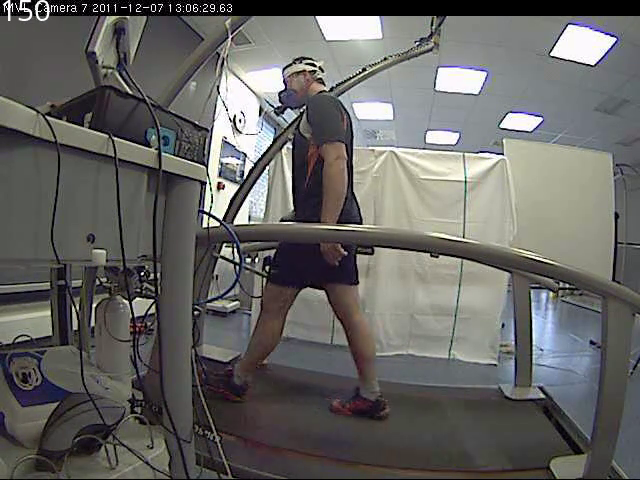
\includegraphics[width=\columnwidth]{./Slike/normal-sv-150.png}
		\caption{stranska slika}
	\end{subfigure}
	~
	\begin{subfigure}{0.45\columnwidth}
		%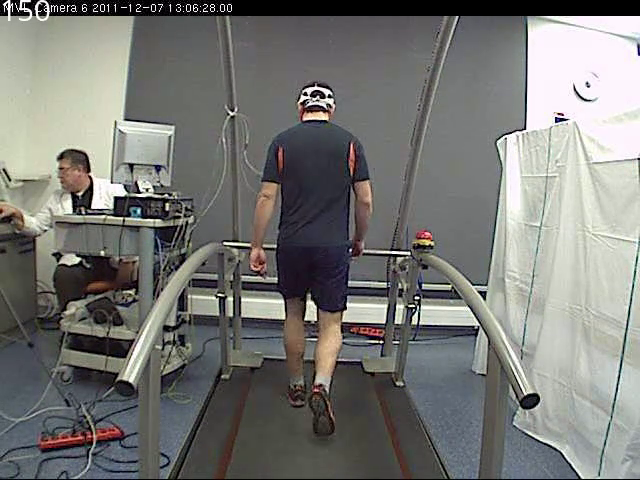
\includegraphics[width=\columnwidth]{./Slike/normal-bv-150.png}
		\caption{hrbtna slika}
	\end{subfigure}
	\caption{Hrbtna in stranska 150. slika RGB posnetkov iz prve serije.}
	\label{fig:primer-posnetka-stage2}
\end{figure}

Snemali smo z dvema Microsoft Xbox Kinect V2 kamerama. Kameri sta bili od tekalne steze oddaljeni približno \SI{2}{m}. Od tal sta bili dvignjeni za približno \SI{1.5}{m}. Postavitev kamer je prikazana na sliki \ref{fig:lab-postavitev-kamer}

\begin{figure}[htb]
	\centering
	\begin{subfigure}[t]{0.45\columnwidth}
		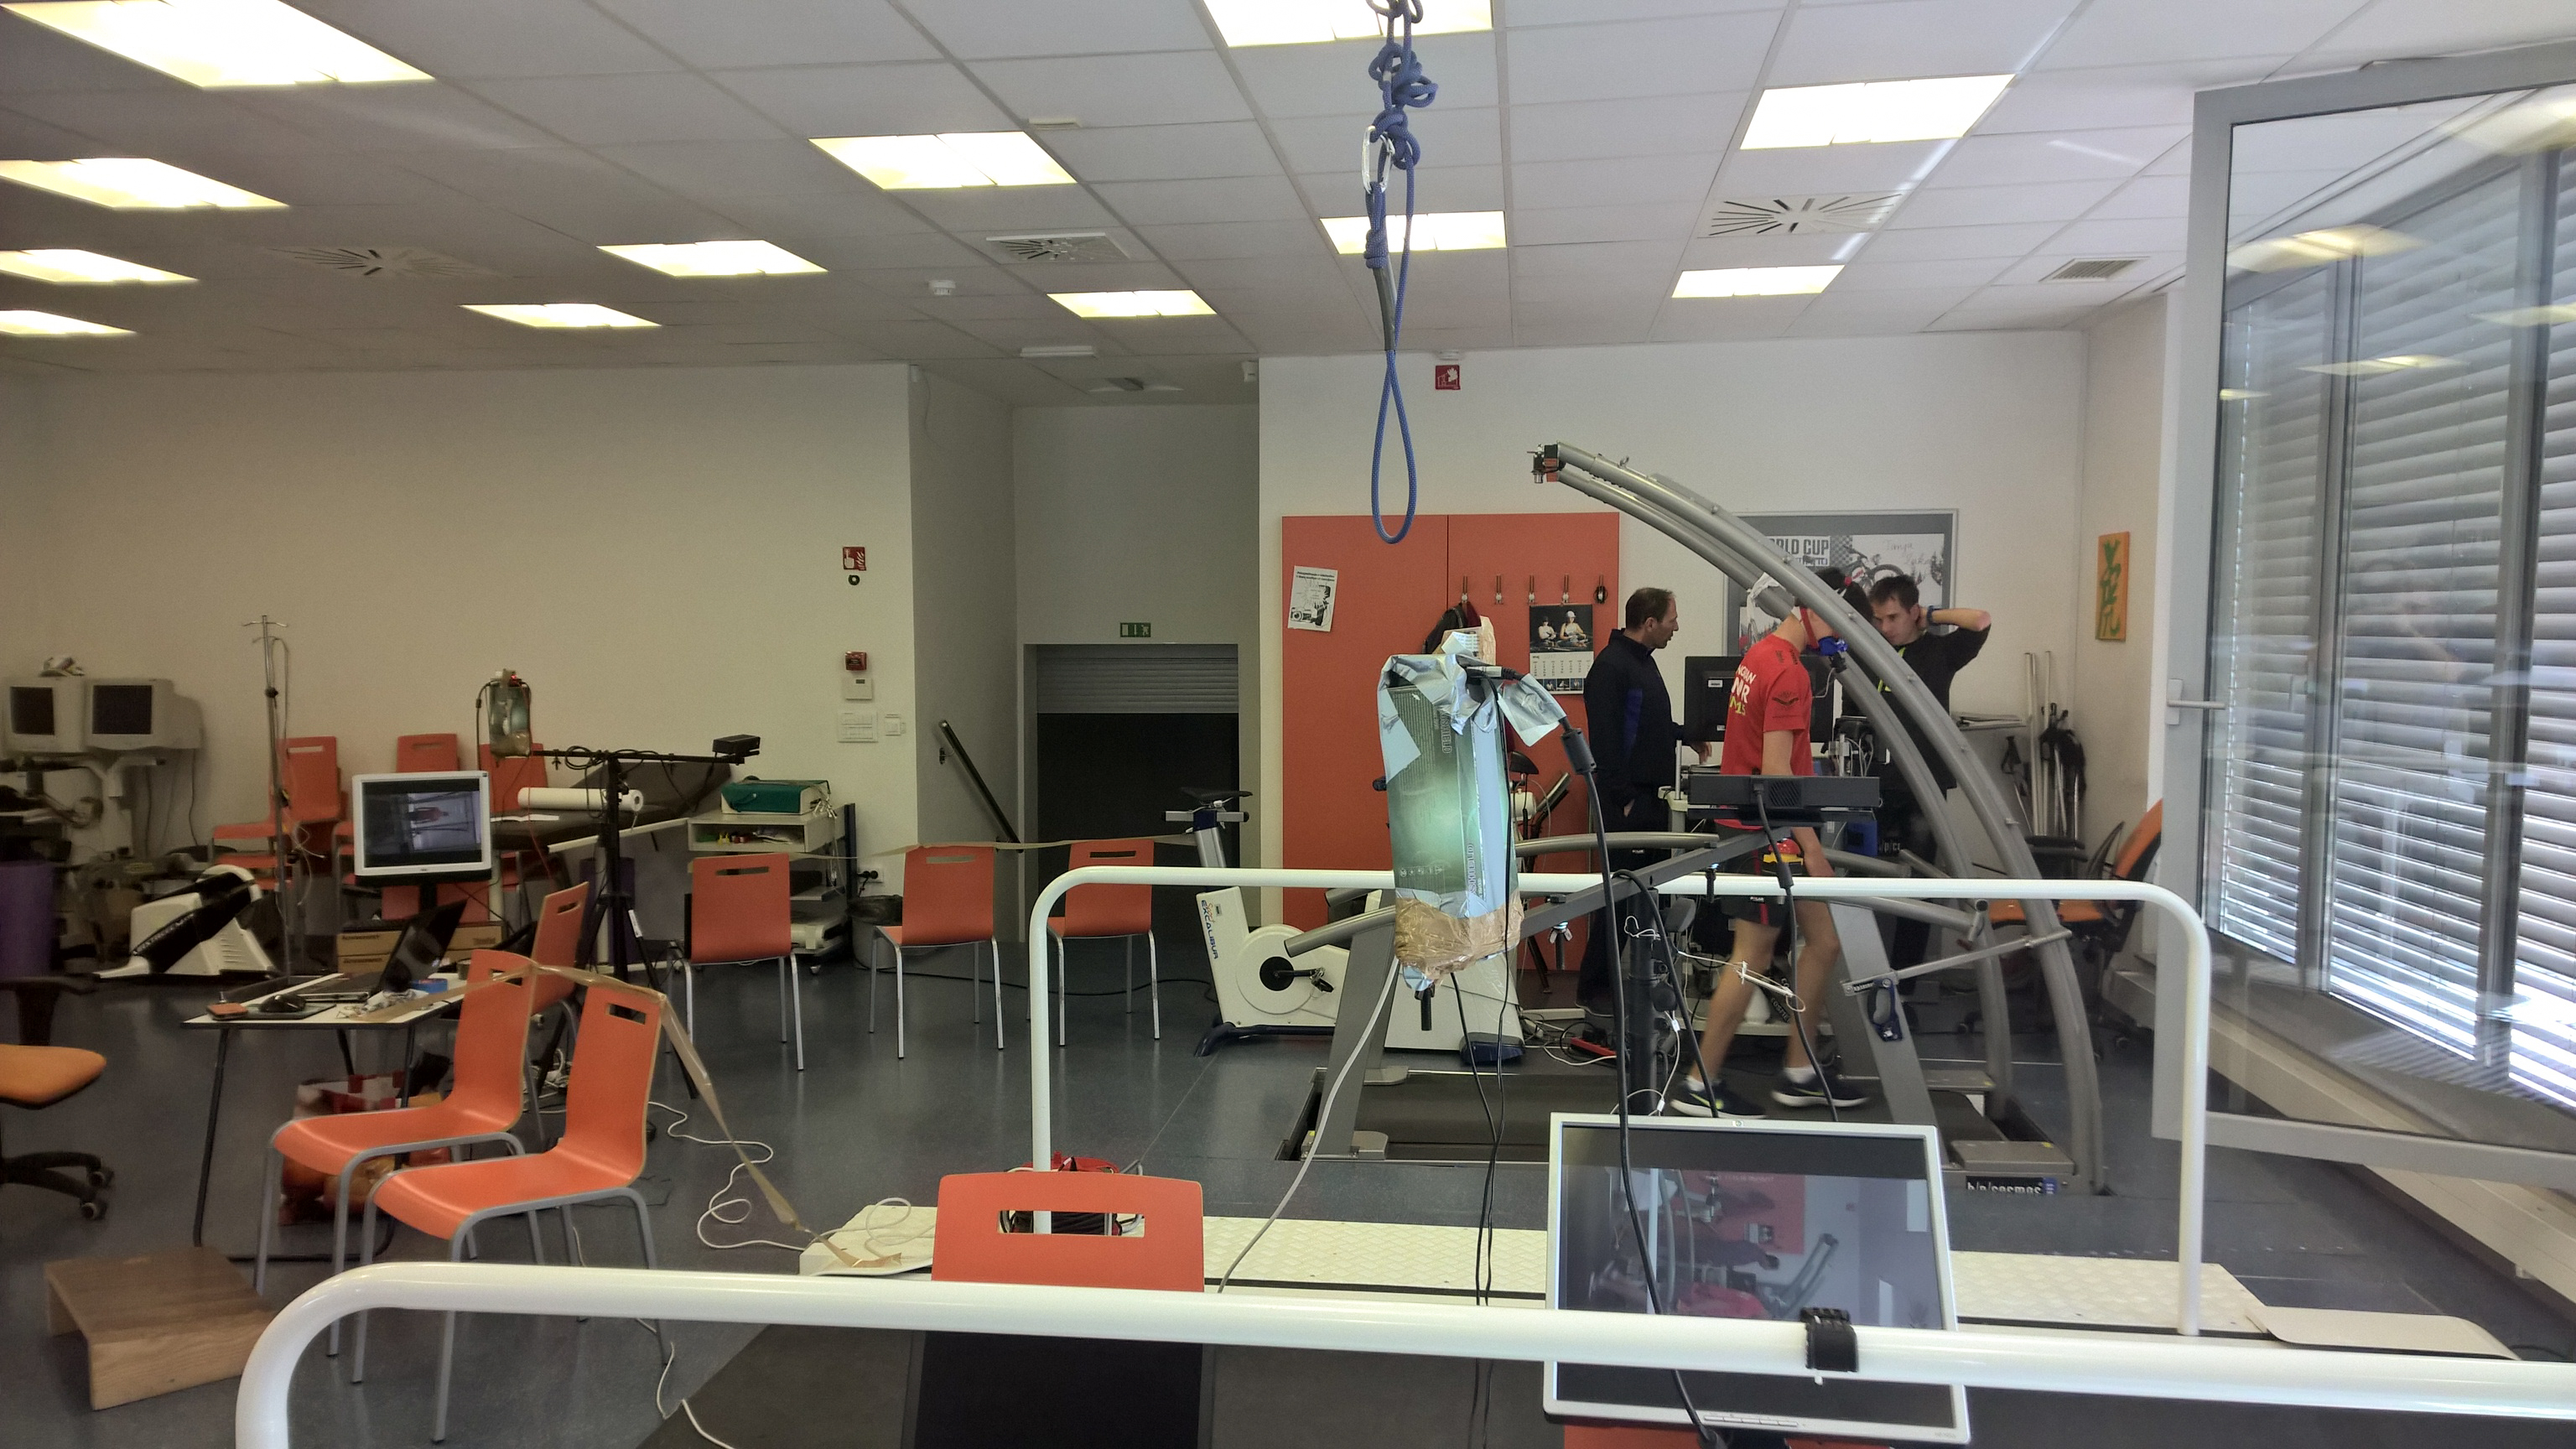
\includegraphics[width=\columnwidth]{./Slike/lab-posnetek-iz-strani-corrected.jpg}
		\caption{Stranski pogled.}
	\end{subfigure}
	~
	\begin{subfigure}[t]{0.45\columnwidth}
		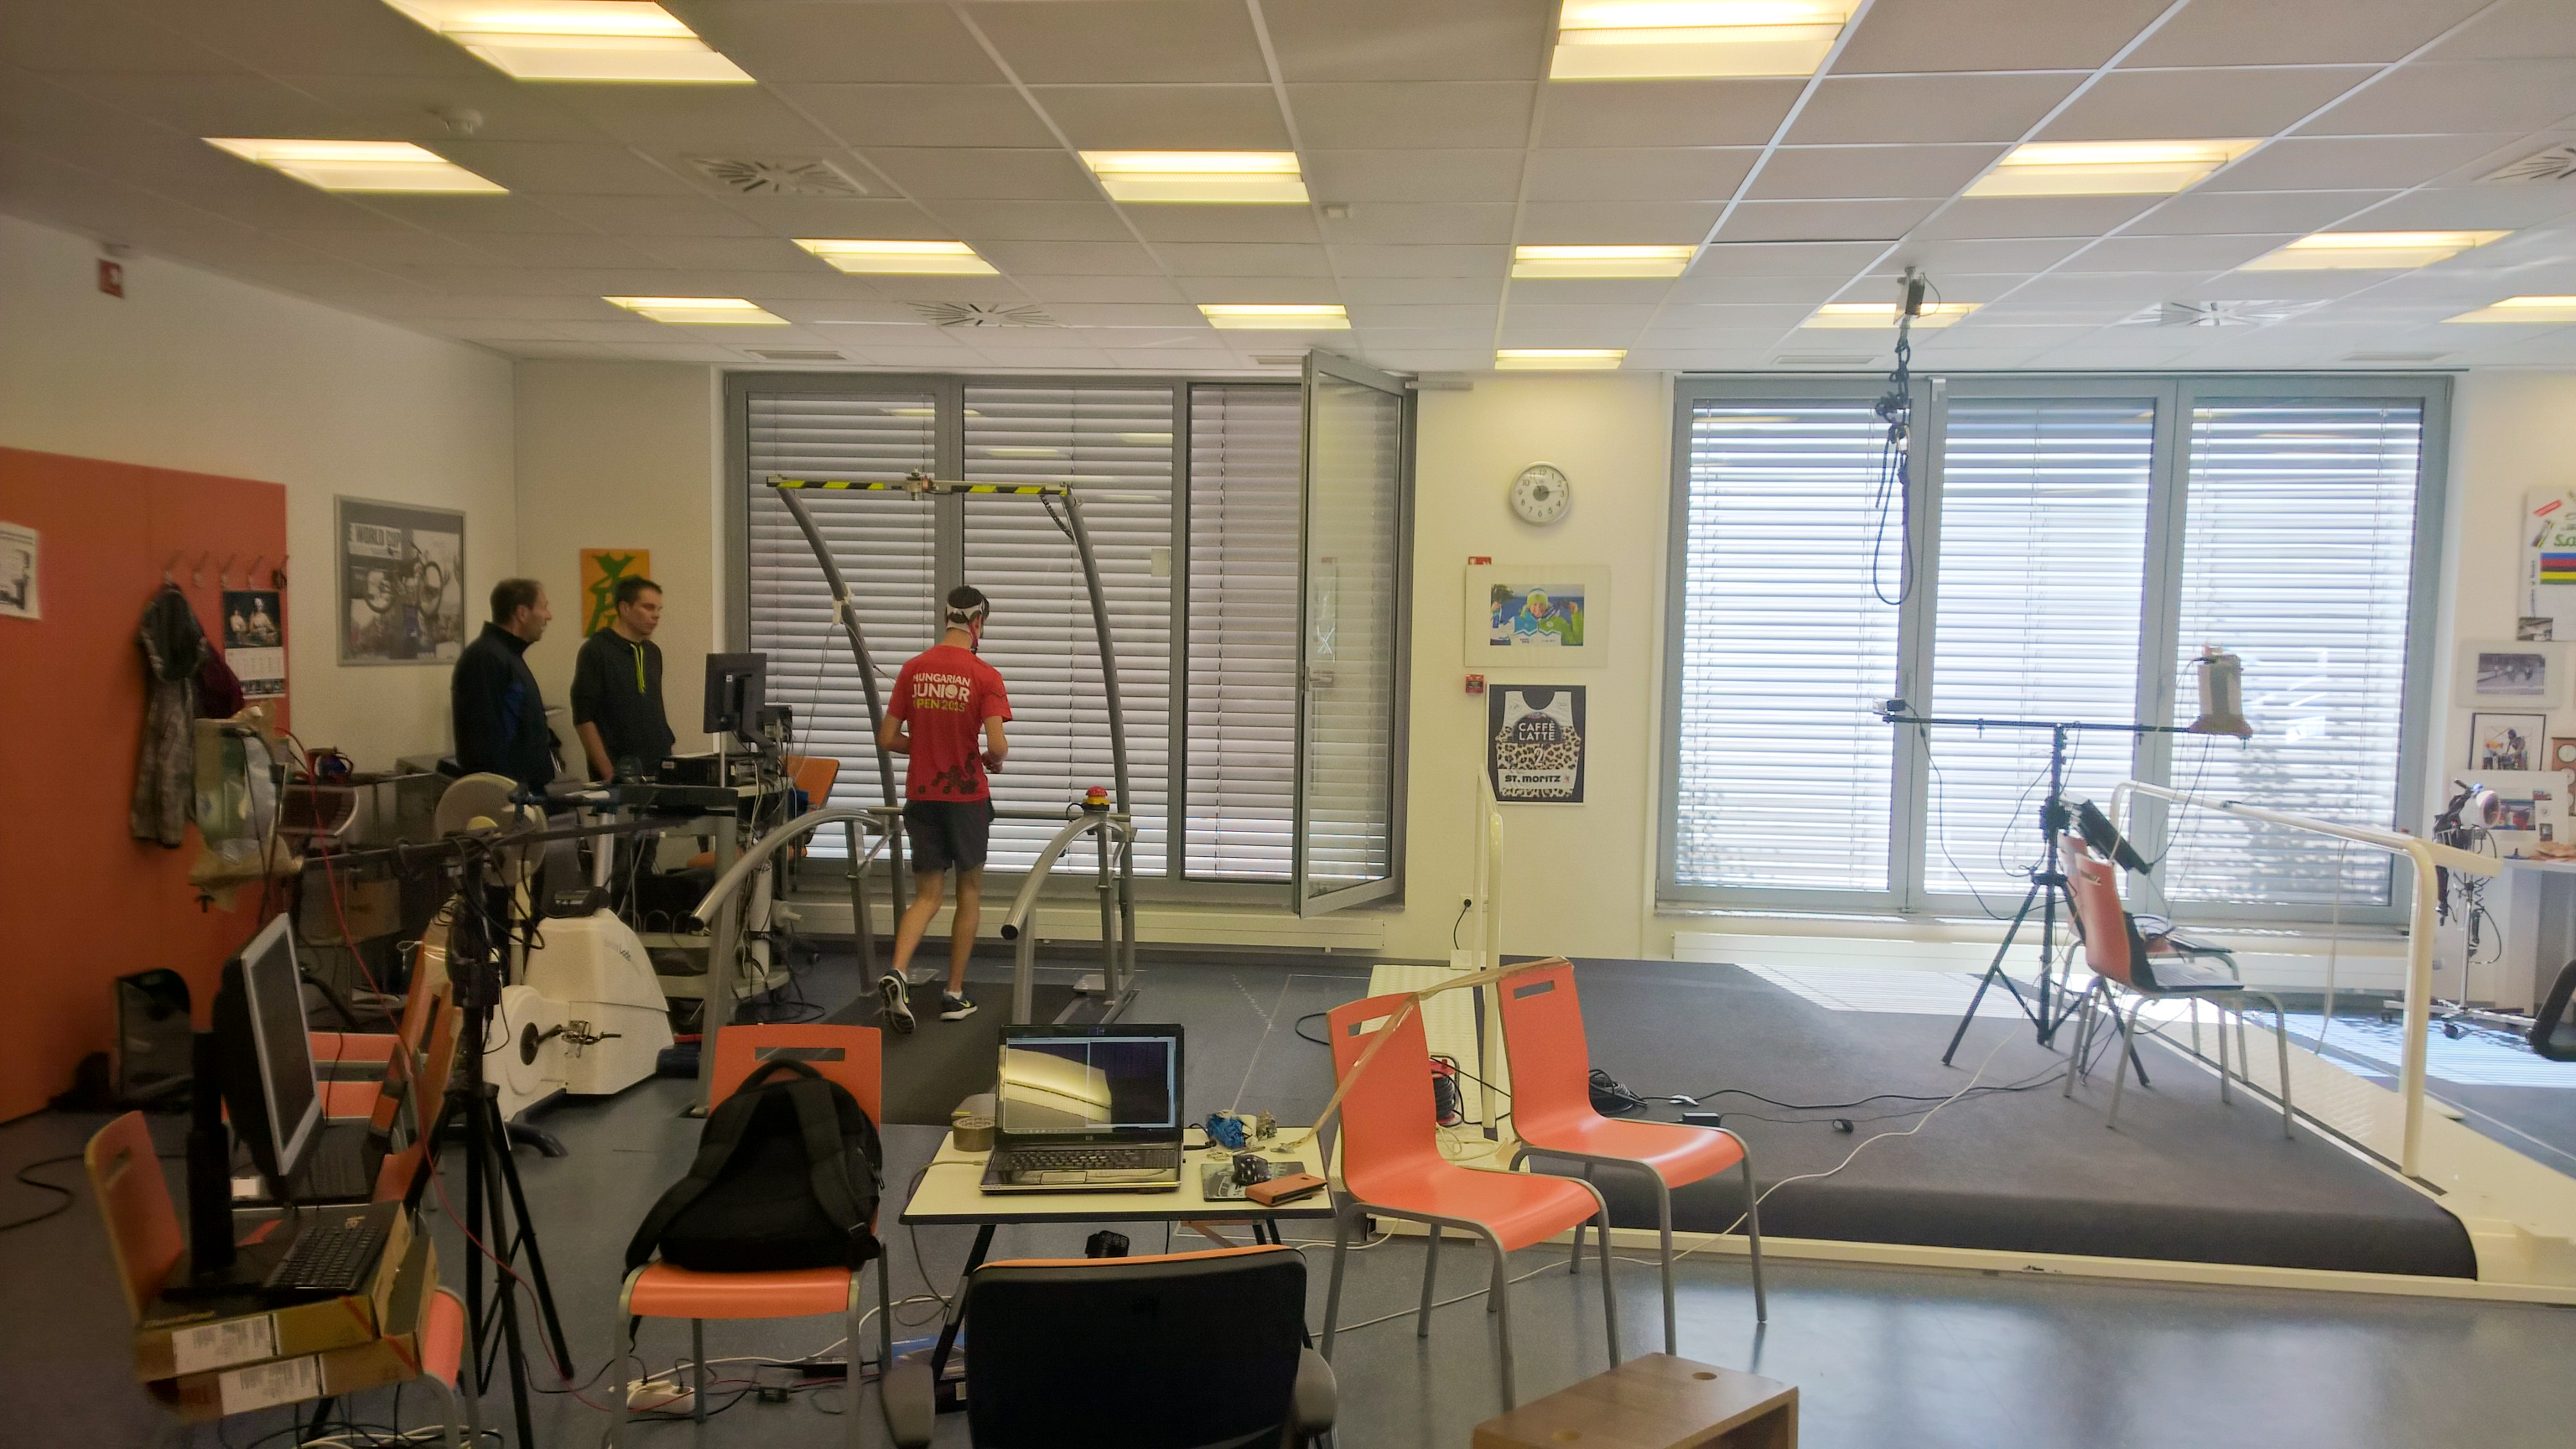
\includegraphics[width=\columnwidth]{./Slike/lab-posnetek-zadaj-corrected.jpg}
		\caption{Hrbtni pogled.}
	\end{subfigure}
	\caption{Stranski in hrbtni pogled postavitve kamer za laboratorijske teste 2. faze.}
	\label{fig:lab-postavitev-kamer}
\end{figure}


Pridobili smo barvne RGB in globinske DEPTH slike. Snemali smo v ločljivosti $512 \times 424$. Hitrost posnetkov je znašala \SI{30}{fps}. Kameri smo časovno sinhronizirali po NTP protokolu.

Obremenilni test smo izvajali s pomočjo sistema za direktno ergospirometrijo tipa ``breath  by breath'' Cosmed K4B2. Uporabili smo  tekočo  preprogo HP Cosmos. Z obremenilnim testom smo pridobili podatke enrgijske porabe šestih različnih merjencev z oznakami: SUBJ1, SUBJ2, SUBJ4, SUBJ7 SUBJ8 in SUBJ9. Vzorčili smo s frekvenco \SI{0.2}{\hertz}.

\subsubsection{Protokol izvajanja meritev}
Test smo pričeli z eno minutnim mirovanjem na tekalni stezi. Sledilo je tri minutno ogrevanje s hitrostjo teka \SI{5}{\km\per\hour}, pri naklonu preproge \SI{0}{\%}. Nadaljevali smo s 3 minutnim tekom s hitrostjo \SI{6}{\km\per\hour}. Po treh minutah smo naklon tekoče preproge  dvignili za \SI{2}{\%} in ga nismo več spreminjali. Po pretečeni minuti na  tretji stopnji (hitrost \SI{6}{\km\per\hour}, naklon \SI{2}{\%}) se je hitrost teka vsaki dve  minuti  povečevala za \SI{1}{\km\per\hour}. Test smo izvajali brez prekinitve do pojava objektivnih oz. subjektivnih razlogov za prekinitev testa. 
%Po koncu testiranja je sledilo še \SI{5}{min} hoje pri  hitrosti \SI{2}{\km\per\hour} ter \SI{0}{\%} naklonu. 
 

\subsubsection{Protokoli postopka procesiranja}
Tako kot pri eksperimentih 1. faze so bile  meritve fizioloških parametrov izvedene z vzorčenjem \SI{0.2}{\hertz}, hitrost posnetkov pa je bila \SI{30}{fps}. Zaradi neskladja frekvenc vzorčenja, smo te interpolirali s pomočjo Matlabove funkcije \texttt{interp1}.

Tokrat smo modele učili po dveh postopkih. Prvi postopek temelji na optičnem toku, drugi pa na prostorskem.

\paragraph{Postopek z optičnim tokom}
Na slikah posnetkov smo merjencem sledili s sledilnikom KCF. Za tako izbrano področje slike smo izračunali optični tok. Primer dobljenega optičnega toka je prikazan na sliki \ref{fig:opticni-tok-stage2}. Sledilo je generiranje HOOF-HAFA deskriptorjev s parametri $N_{HOOF} = 60$ in $N_{HAFA} = 60$. HAFA deskriptorje smo normalizirali z vrednostmi amplitudnih faktorjev $f_A$, ki so zbrani v tabeli \ref{tab:fa-merjenci}.

\begin{figure}[htb]
	\centering
    \caption{Optični tok}
	\label{fig:opticni-tok-stage2}
\end{figure}

\begin{table}[htb]
	\centering
	\begin{tabular}{l l S[table-format=3.3]}
		\toprule
		\textbf{Pogled} & \textbf{Merjenec} & \thead{$\mathbf{f_A}$} \\
		\midrule
		\multirow{7}{*}{hrbtni}
		&1&208.557\\
		&2&179.011\\
		&4&225.568\\
		&7&195.133\\
		&8&209.991\\
		&9&182.003\\
		&10&207.002\\
		\midrule
		\multirow{7}{*}{stranski}
		&1&236.985\\
		&2&163.957\\
		&4&196.461\\
		&7&205.760\\
		&8&190.253\\
		&9&178.16\\
		\bottomrule
	\end{tabular}
	\caption[Faktor amplitud za posamezne merjence pri različnem pogledu]{Faktor amplitud za posamezne merjence pri različnem pogledu.}
	\label{tab:fa-merjenci}
\end{table}

\begin{figure}[htb]
	\centering
	\begin{tikzpicture}
% LAYERS
\pgfdeclarelayer{bg}
\pgfsetlayers{bg,main}
\tikzset{
    between/.style args={#1 and #2}{
         at = ($(#1)!0.5!(#2)$)
    }
}

% NODES
\node (slika) [input] at (0,0) {Slika\\$I(x,y)$};
\node (tracker) [block, right= of slika] {KCF\\sledilnik};
%\node (tarca) [block, right= of tracker] {Področje tarče};

\node (of) [block, right= of tracker] {Optični\\tok $\vec{w}$};
\node (hoof) [block, right= of of] {HOOF-HAFA\\deskriptorji $\vec{x}(t)$};


\node (ucenje) [block, right=of hoof] {\nurbf};
\node (kalman) [block, right= of ucenje] {Gaussov\\filter};


\node (rezultat) [output, right= of kalman] {Rezultat};

% arrows
\draw [arrow] (slika) -- (tracker);
\draw [arrow] (tracker) -- (of);
%\draw [arrow] (tarca) -- (of);
\draw [arrow] (of) -- (hoof);
\draw [arrow] (hoof) -- (ucenje);
\draw [arrow] (ucenje) -- (kalman);
\draw [arrow] (kalman) -- (rezultat);
\end{tikzpicture}
	\caption{Diagram postopka procesiranja z optičnim tokom za eksperimente 2. faze.}
	\label{fig:diagram-procesiranja-of-stage2}
\end{figure}

\paragraph{Postopek s prostorskim tokom}
Na slikah posnetkov smo merjencem sledili s sledilnikom DS-KCF. Za tako izbrano področje slike smo izračunali prostorski tok. Primer dobljenega optičnega toka je prikazan na sliki \ref{fig:prostorski-tok-stage2}. Sledilo je generiranje HOOF-HAFA deskriptorjev s parametri $N_{HOOF} = 60$ in $N_{HAFA} = 60$. HAFA deskriptorjev  nismo normalizirali, ker smo histograme pridobili iz podatkov z metričnimi enotami. 

\begin{figure}[htb]
	\centering
    \caption{Prostorski tok}
	\label{fig:prostorski-tok-stage2}
\end{figure}

\begin{figure}[htb]
	\centering
	\begin{tikzpicture}
% LAYERS
\pgfdeclarelayer{bg}
\pgfsetlayers{bg,main}
\tikzset{
	between/.style args={#1 and #2}{
		at = ($(#1)!0.5!(#2)$)
	}
}

% NODES
\node (slika) [input] at (0,0) {Slika\\$I(x,y)$};
\node (tracker) [block, right= of slika] {DS-KCF\\sledilnik};
%\node (tarca) [block, right= of tracker] {Področje\\ tarče $x^{p}$};

\node (of) [block, right= of tracker] {Prostorski\\ tok};
\node (hoof) [block, right= of of] {HOOF-HAFA\\deskriptorji};


\node (ucenje) [block, right=of hoof] {\nurbf};
\node (kalman) [block, right= of ucenje] {Gaussov\\ filter};


\node (rezultat) [output, right= of kalman] {Rezultat};

% arrows
\draw [arrow] (slika) -- (tracker);
\draw [arrow] (tracker) -- (of);
%\draw [arrow] (tarca) -- (of);
\draw [arrow] (of) -- (hoof);
\draw [arrow] (hoof) -- (ucenje);
\draw [arrow] (ucenje) -- (kalman);
\draw [arrow] (kalman) -- (rezultat);
\end{tikzpicture}
	\caption{Diagram postopka procesiranja s prostorskim tokom za eksperimente 2. faze.}
	\label{fig:diagram-procesiranja-sf-stage2}
\end{figure}
 
Modele obeh postopkov smo učili s postopkom \nurbf, kjer smo za Gaussov filter uporabili $\sigma=5$ in za največje število podpornih vektorjev $\numax =0.5$ (\SI{50}{\%} podpornih vektorjev). Podobno kot v eksperimentih 1. faze smo tudi tu naučili \num{6} elementarnih modelov, in sicer: \textit{eem} modele, ki predvidevajo porabo energije v \si{\kcal\per\min}, \textit{sv} modele za stransko kamero in \textit{bv} modele za hrbtno kamero ter \textit{lag} modele z upoštevanjem časovne zakasnitve.

Vse tipe eksperimentov smo križno testirali glede na enak tip eksperimenta, le z drugim zornim kotom kamere. Uporabljen zorni kot kamere za križno testiranje je v imenih modelov zapisan v oklepajih.  Rezultate smo filtrirali z Gaussovim jedrom $\sigma=5$. 

Modele smo testirali po treh različnih protokolih. S prvim protokolom smo preverjali neodvisnost od časovnega povečevanja porabe, z drugim pa ravno obratno. S tretjim protokolom smo želeli pokazati delovanje posplošenega modela na različnih merjencih.


\paragraph{Protokol 1.}
Za testne vzorce vzamemo vsak 3. vzorec fiziološkega parametra in slike iz posameznega posnetka. Ostale vzorce uporabimo pri učenju. Rezultate vseh 6 meritev povprečimo.

\paragraph{Protokol 2.}
Za učne vzorce izberemo prvih \SI{70}{\%} vzorce in za testne naslednjih \SI{30}{\%}. Rezultate vseh 6 meritev povprečimo.

\paragraph{Protokol 3.}
Uporabimo protokol 1, pri čemer učimo na prvih štirih meritvah in testiramo na zadnjih dveh. Rezultata povprečimo.

\subsubsection{Določitev zakasnitve fiziološkega odziva}
Določitve zakasnitve fiziološkega odziva smo se, glede na eksperimente 1. faze, tu lotili nekoliko drugače. Na podlagi protokola izvajanja meritev, smo pridobili podatke eno minutnega mirovanja posameznega merjenca z vzorčno frekvenco \SI{0.2}{\hertz}. Kljub temu, da je signal v stacionarnem stanju, je nihajoč zaradi narave fiziologije. Signal mirovanja smo interpolirali na vzorčno frekvenco \SI{1}{\hertz}. Določili smo mu srednjo vrednost in vrednost treh standardnih odklonov. S tem smo dobili interval nedoločenosti, v katerem ne moremo določiti ali je pri spremembi amplitude signala prišlo zaradi fizioloških dejavnikov ali zaradi dejanskega odziva na vzbujalni signal. 

Na podlagi slik \ref{fig:lag-estimation-stage2}, smo zakasnitev za posamezno meritev določili kot časovni interval od trenutka spremembe hitrosti tekalne steze do trenutka, ko je bila vrednost fiziološkega parametra prvič nad intervalom nedoločenosti. Zakasnitev smo, zaradi treh standardnih odklonov, lahko določili s \SI{99.73}{\%} zagotovostjo za posameznega merjenca. Zakasnitve vseh merjencev smo povprečili in dobili vrednost \SI{26}{\s} za energijsko porabo.

\begin{figure}[!htbp]
	\centering
	\begin{subfigure}[t]{0.45\columnwidth}
		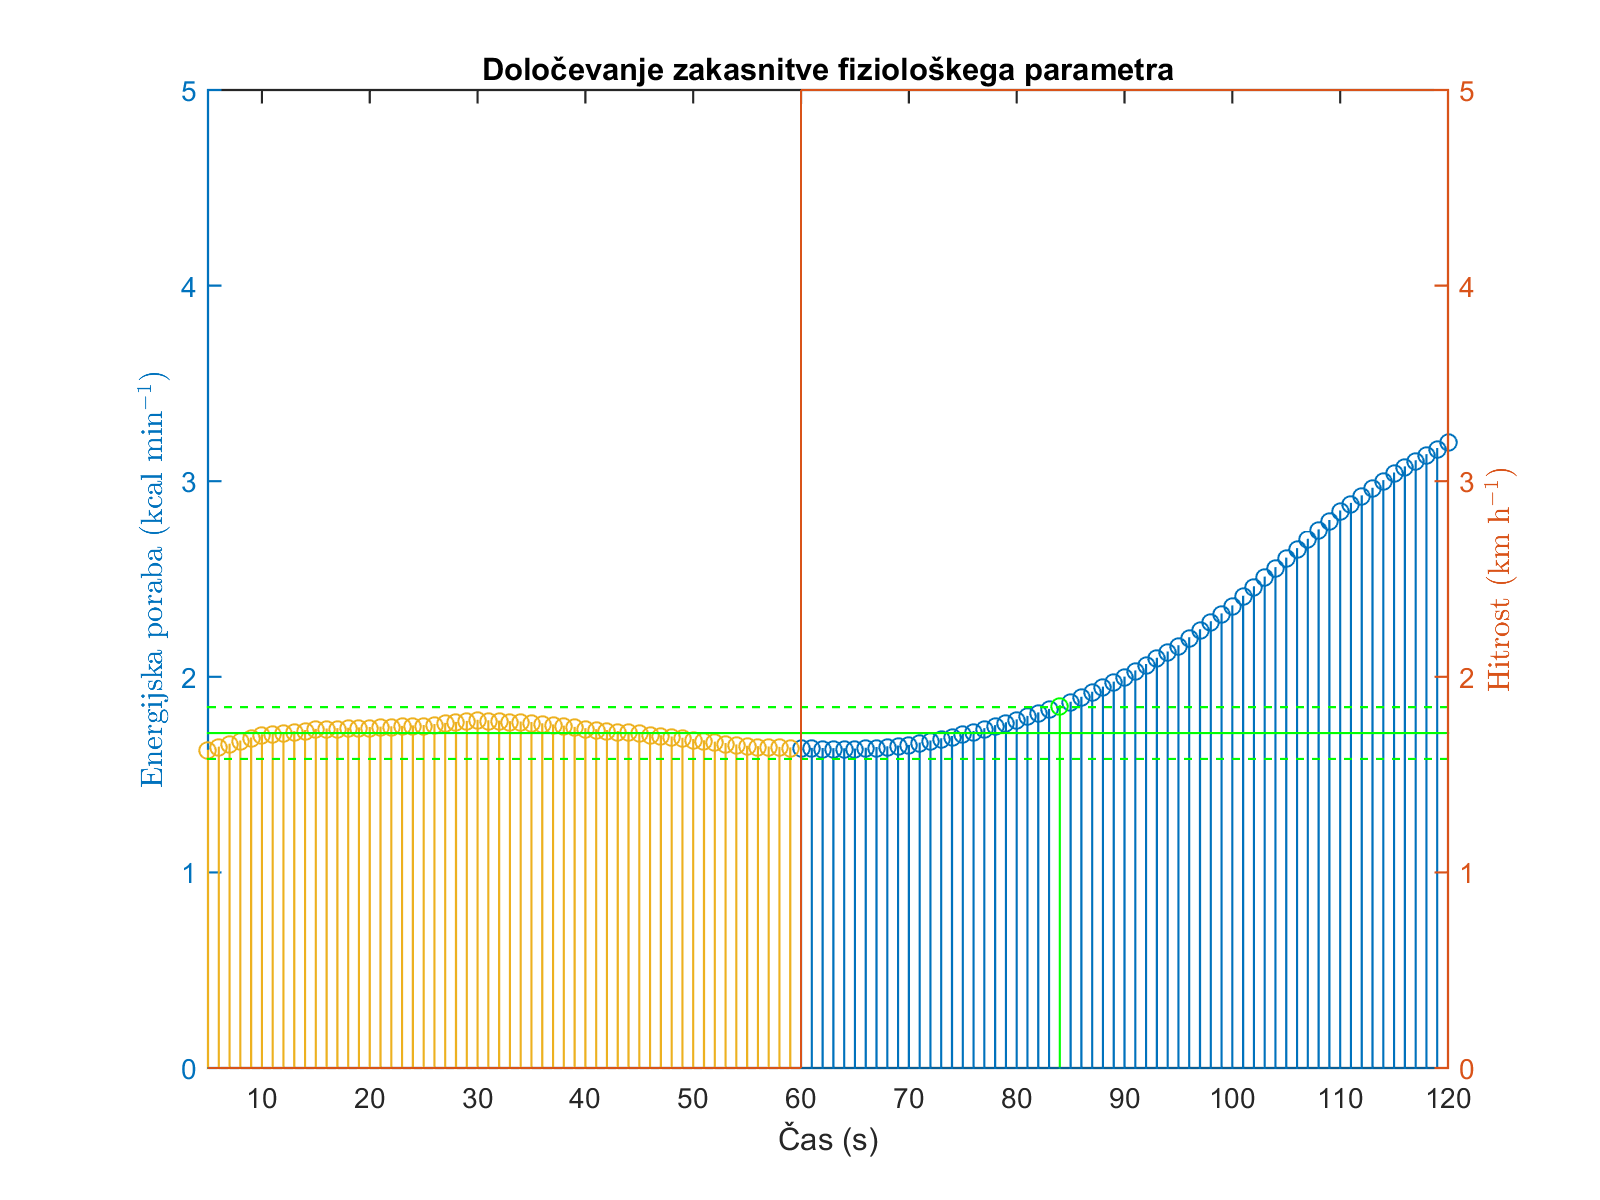
\includegraphics[width=\columnwidth]{./Slike/lag-estimation-1-eem.png}
		\caption{Zakasnitev za subjekt 1.}
		\label{fig:lag-estimation-1-eem}
	\end{subfigure}
	~
	\begin{subfigure}[t]{0.45\columnwidth}
		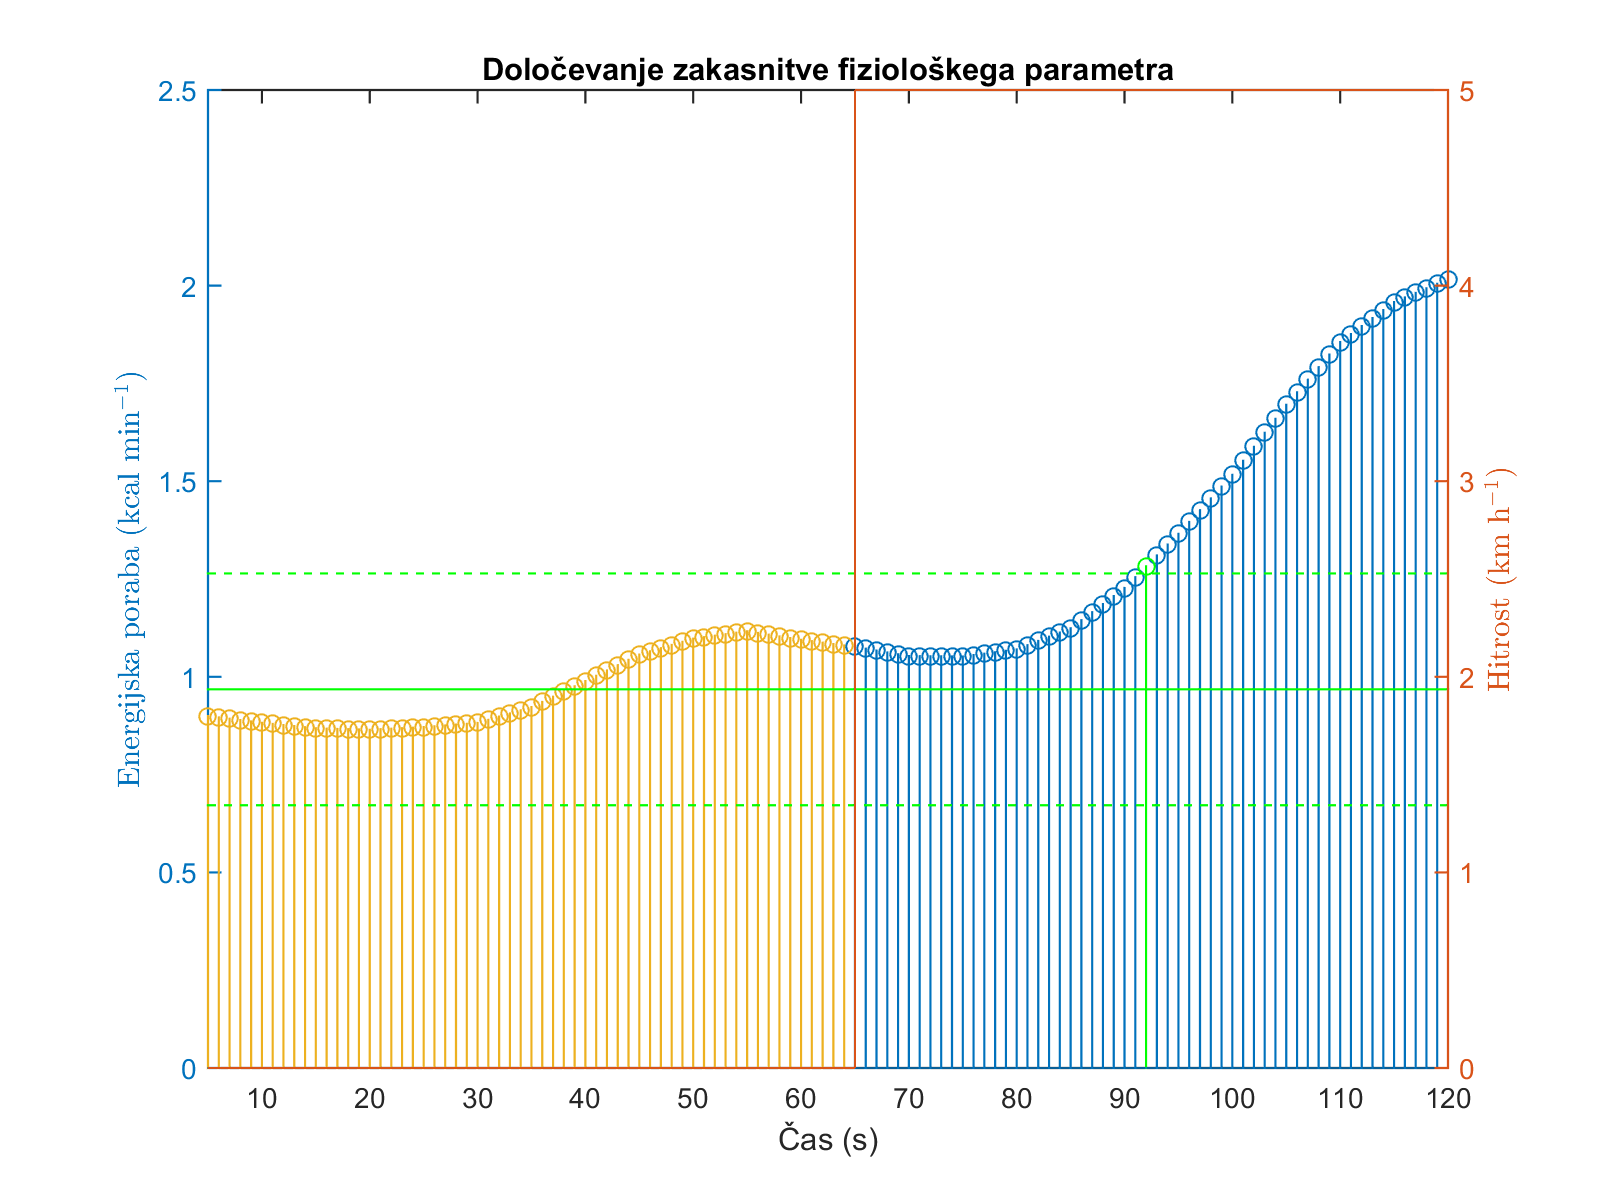
\includegraphics[width=\columnwidth]{./Slike/lag-estimation-2-eem.png}
		\caption{Zakasnitev za subjekt 2.}
		\label{fig:lag-estimation-2-eem}
	\end{subfigure}
	~
	\begin{subfigure}[t]{0.45\columnwidth}
		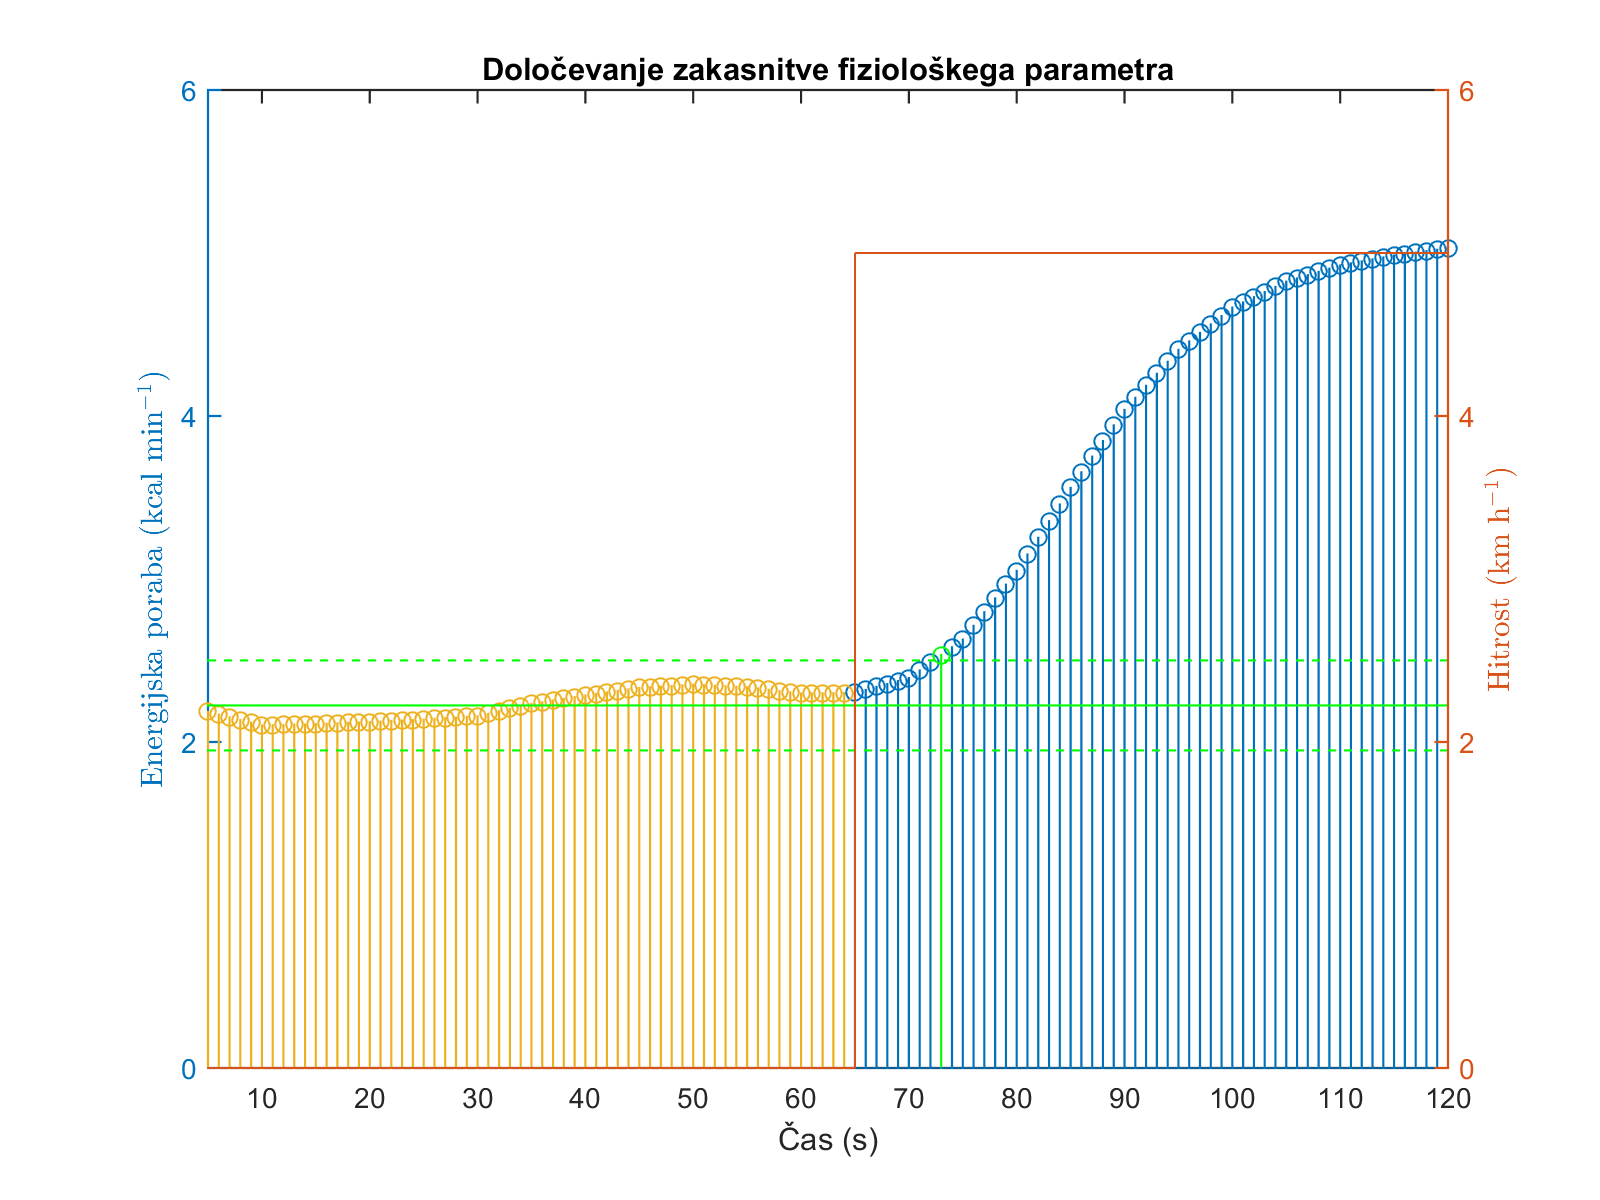
\includegraphics[width=\columnwidth]{./Slike/lag-estimation-3-eem.png}
		\caption{Zakasnitev za subjekt 3.}
		\label{fig:lag-estimation-3-eem}
	\end{subfigure}
	~
	\begin{subfigure}[t]{0.45\columnwidth}
		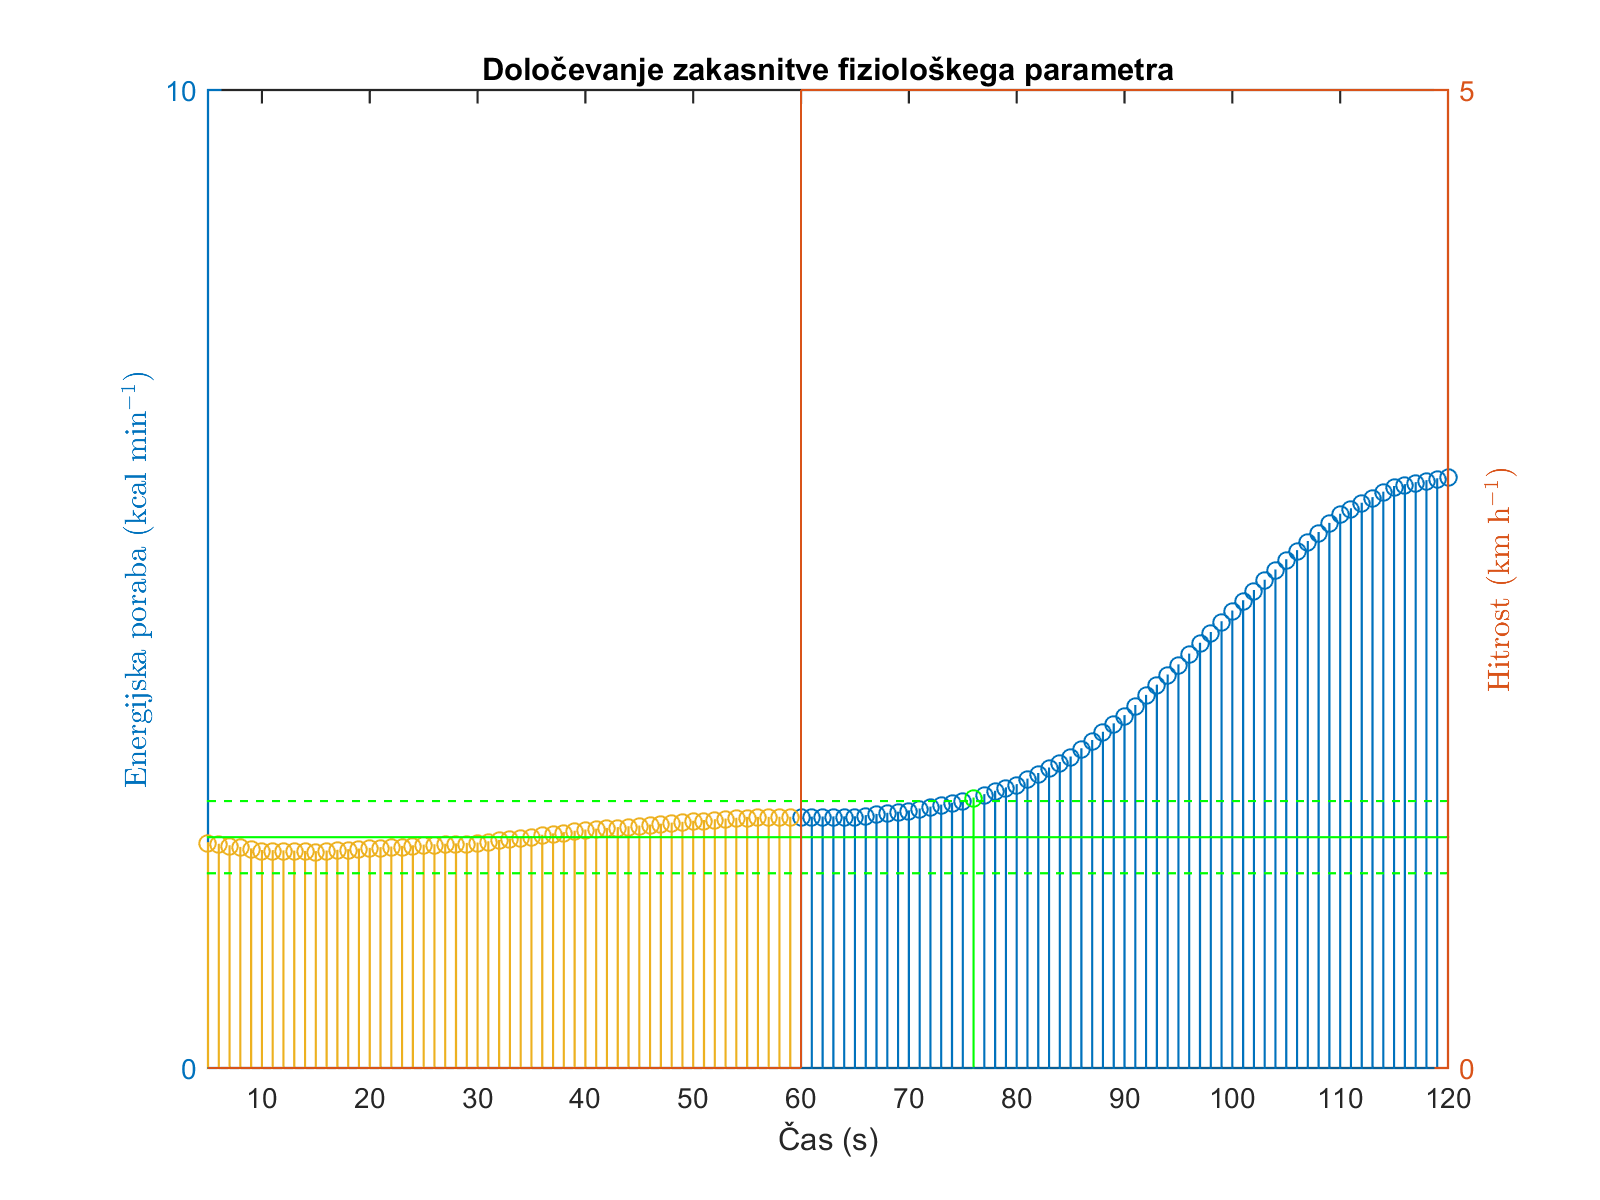
\includegraphics[width=\columnwidth]{./Slike/lag-estimation-4-eem.png}
		\caption{Zakasnitev za subjekt 4.}
		\label{fig:lag-estimation-4-eem}
	\end{subfigure}
	~
	\begin{subfigure}[t]{0.45\columnwidth}
		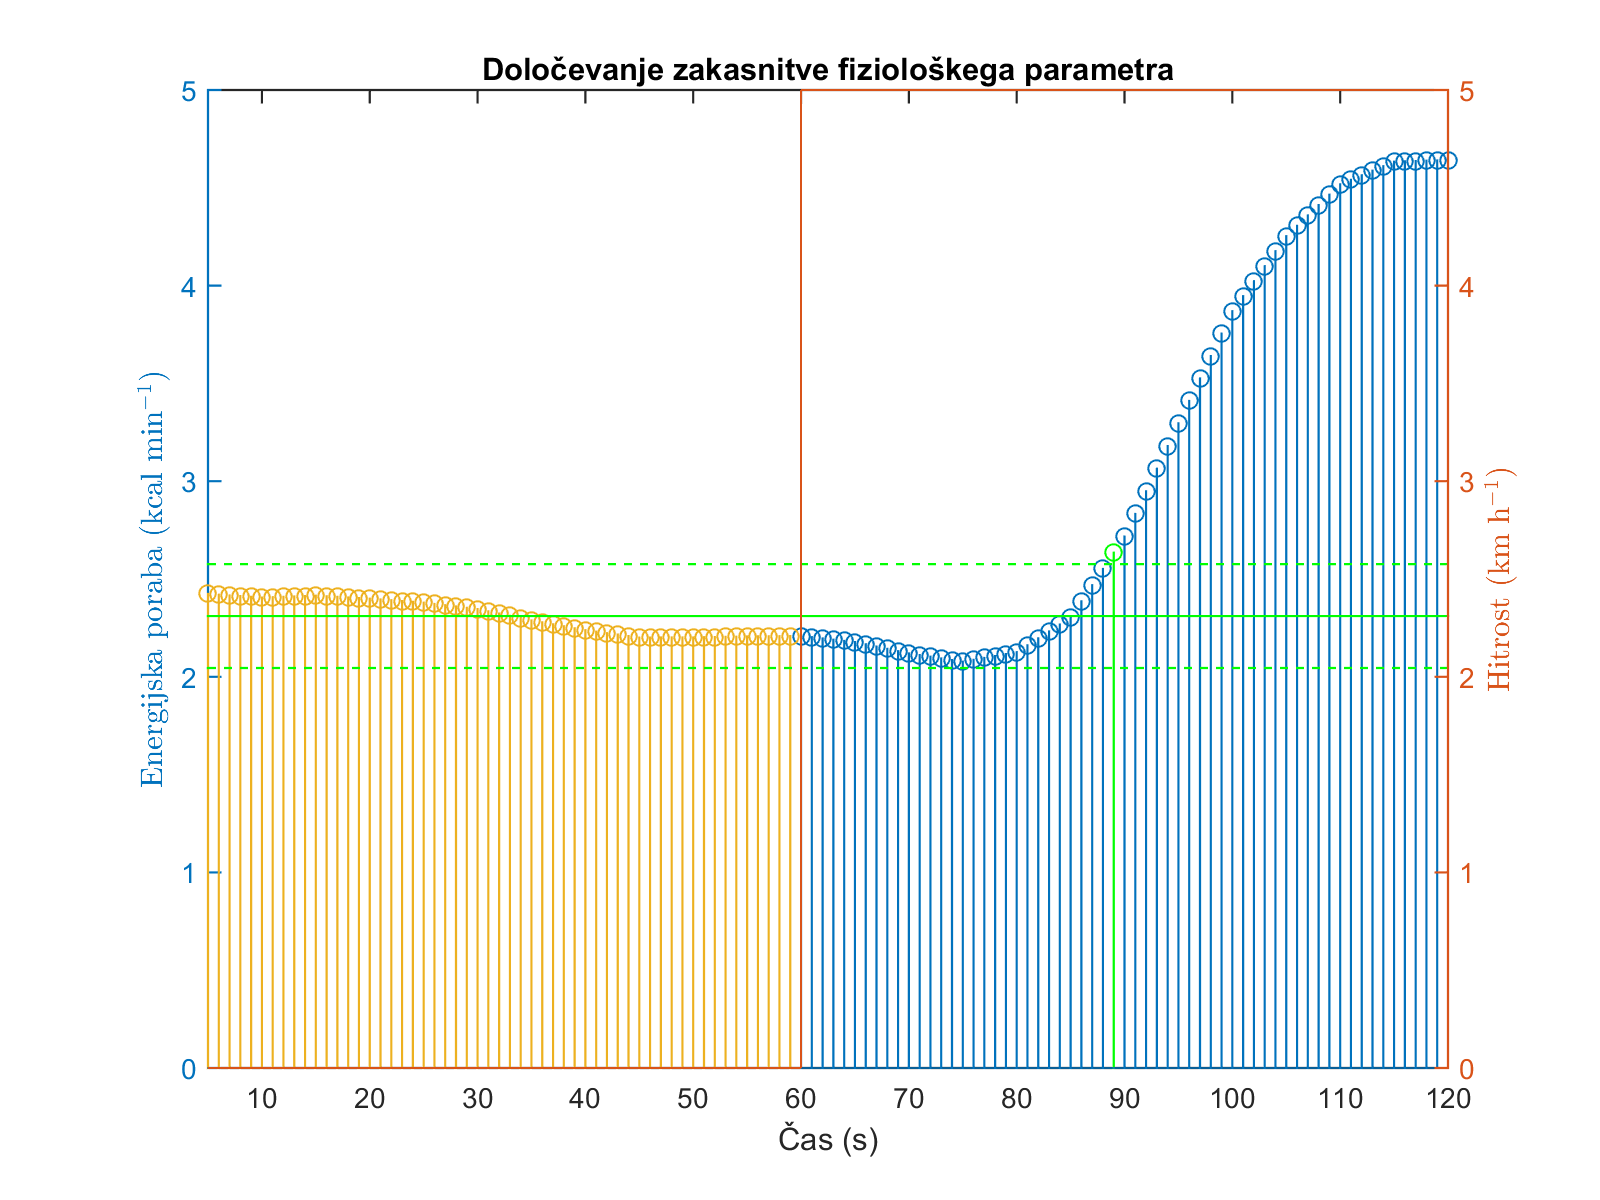
\includegraphics[width=\columnwidth]{./Slike/lag-estimation-5-eem.png}
		\caption{Zakasnitev za subjekt 5.}
		\label{fig:lag-estimation-5-eem}
	\end{subfigure}
	~
	\begin{subfigure}[t]{0.45\columnwidth}
		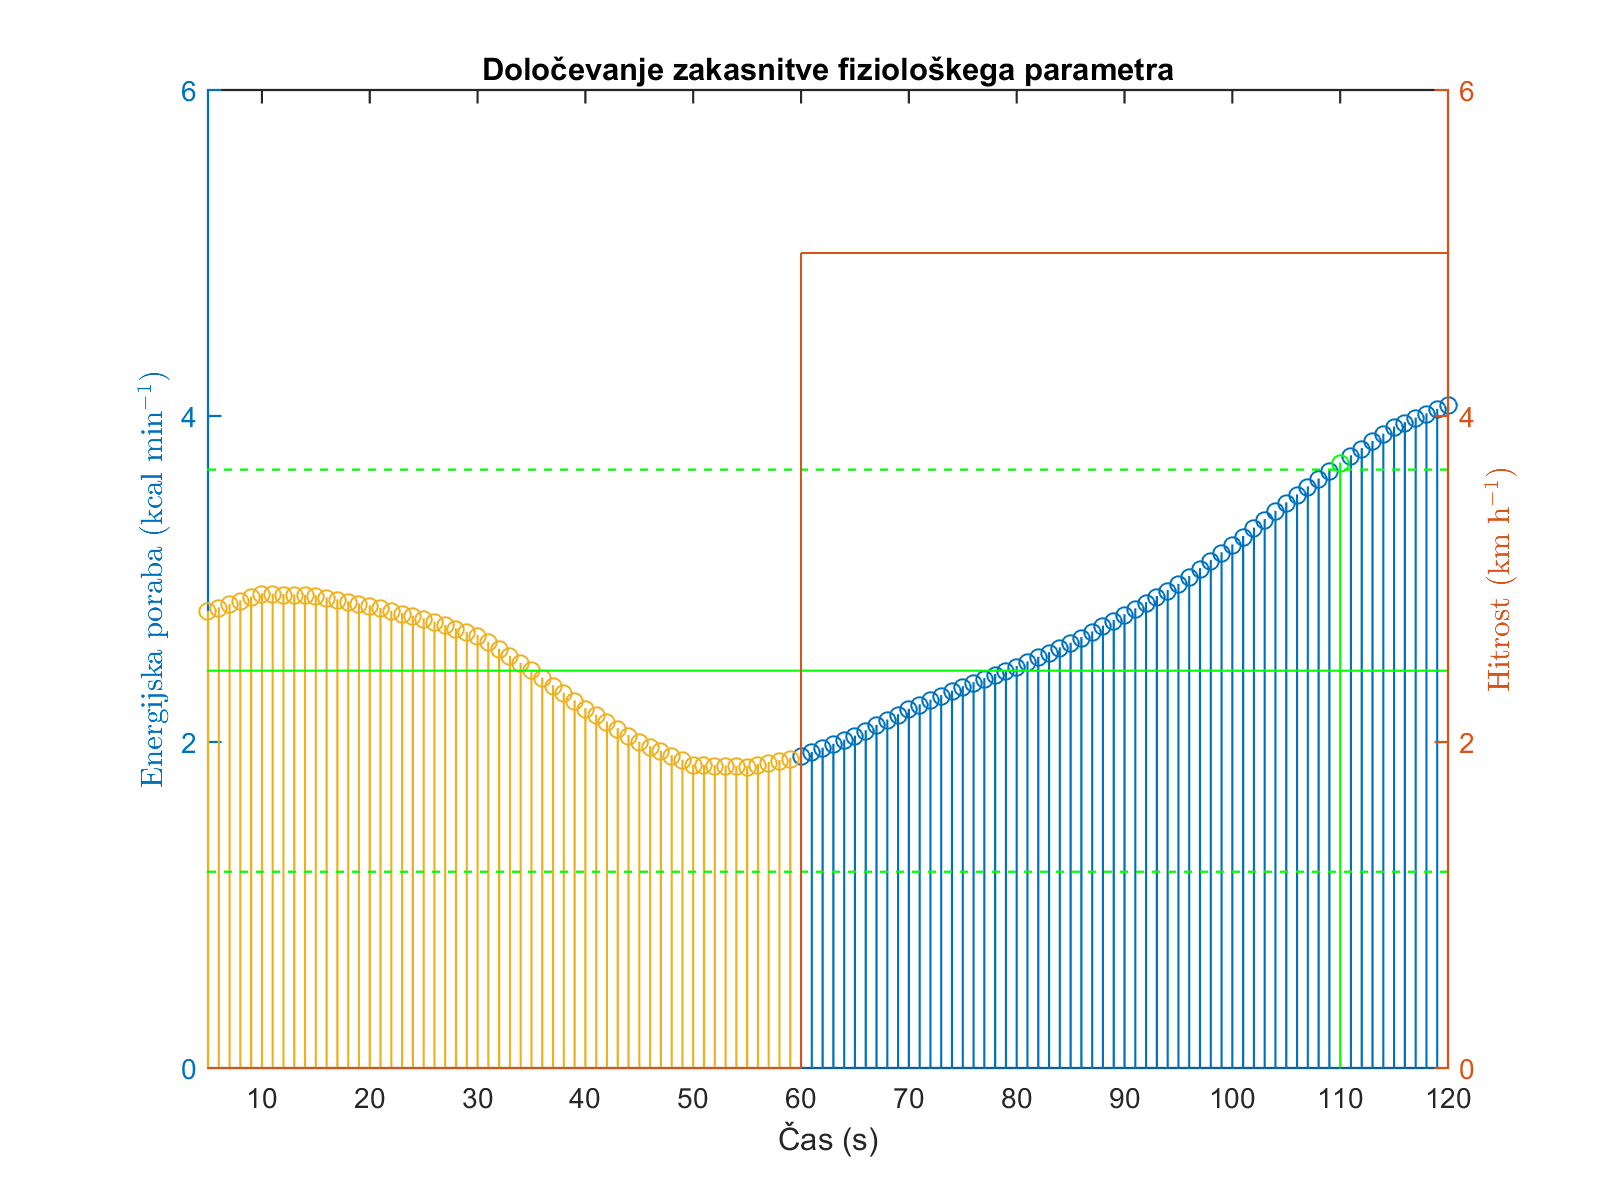
\includegraphics[width=\columnwidth]{./Slike/lag-estimation-6-eem.png}
		\caption{Zakasnitev za subjekt 6.}
		\label{fig:lag-estimation-6-eem}
	\end{subfigure}
	\caption{}
	\label{fig:lag-estimation-stage2}
\end{figure}










\subsection{Terenski eksperimenti}
Pri terenskih eksperimentih smo postopek z optičnim tokom in postopek s prostorskim tokom preverili še v realističnem okolju. Šest igralcev je igralo squash igro z dvema setoma. Tako smo pridobili podatke za 3 igre, ki so trajale \SI{16}{min} \SI{14}{min} in \SI{11}{min}. Postopki procesiranja in protokoli procesiranja so enaki kot v laboratorijskih eksperimentih 2. faze. 

\begin{figure}[htb]
	\centering
	\begin{subfigure}{0.45\columnwidth}
		%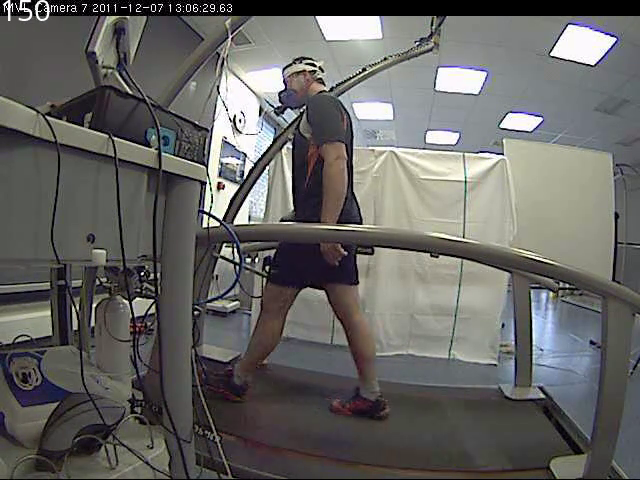
\includegraphics[width=\columnwidth]{./Slike/normal-sv-150.png}
		\caption{stranska slika}
	\end{subfigure}
	~
	\begin{subfigure}{0.45\columnwidth}
		%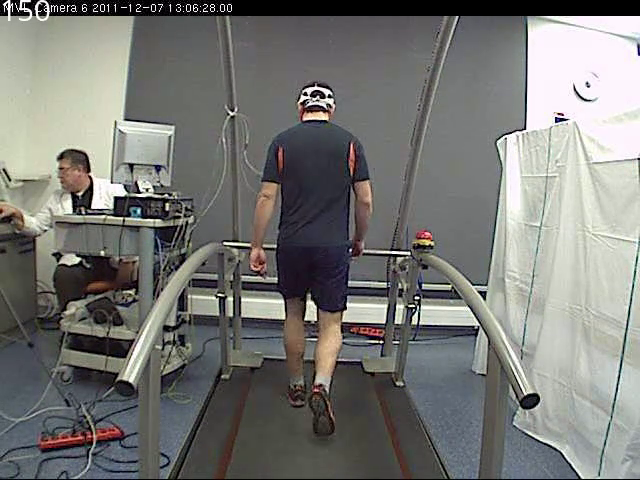
\includegraphics[width=\columnwidth]{./Slike/normal-bv-150.png}
		\caption{hrbtna slika}
	\end{subfigure}
	\caption{Hrbtna in stranska 150. slika RGB posnetkov iz prve serije.}
	\label{fig:primer-posnetka-teren}
\end{figure}

\paragraph{Pridobivanje podatkov.}
Igrišče smo snemali z dvema Microsoft Xbox Kinect V2 kamerama, ki sta bili oddaljeni ena od druge za približno \SI{2}{m}. Vsaka kamera je pokrivala svojo polovico igrišča. Razdalja od tal je znašala približno \SI{3}{m}. Kameri sta bili tako pozicionirani nad zaščitnim steklom. S tem nismo dobili odbojev laserskih žarkov, ki so namenjeni za pridobivanje globinske slike. Kot $\theta$ (rotacija okoli x osi) je bil približno $30\stopinj$ tako, da so kamere pokrivale prvo polovico igrišča do linije serviranja.

Pridobili smo barvne RGB in globinske DEPTH slike. Snemali smo v ločljivosti $512 \times 424$. Hitrost posnetkov je znašala \SI{30}{fps}. Kameri smo časovno sinhronizirali po NTP protokolu.

Fiziološke parametre smo pridobili s pomočjo prenosnega sistema za direktno ergospirometrijo tipa ``breath  by breath'' Cosmed K4B2. Frekvenca vzorčenja se je spreminjala, v povrečju pa je znašala \SI{0.5}{\hertz}. S testom smo pridobili podatke energijske porabe šestih različnih merjencev z oznakammi: SUBJ1, SUBJ2, SUBJ7, SUBJ8, SUBJ9 in SUBJ10.

\paragraph{Protokol izvajanja meritev.}
Posamezno igro smo pričeli s 5 minutnim ogrevalnim tekom. Sledilo je igranje na dva seta do 10 dobljenih točk z upoštevanjem dveh točk razlike. Med setoma so igralci počivali 2 minute. Ogrevanja in počivanja s kamerami nismo merili. Seta posamezne igre smo združili v en posnetek.
